% nSIEguide.tex
% v4.0 released December 2014

\documentclass[]{article}
\usepackage{graphicx}
\usepackage{epstopdf}% To incorporate .eps illustrations using PDFLaTeX, etc.
\usepackage{subfigure}% Support for small, `sub' figures and tables
%\usepackage{natbib}% Citation support using natbib.sty
%\usepackage[longnamesfirst,sort]{natbib}% Citation support using natbib.sty
%\bibpunct[, ]{(}{)}{;}{a}{,}{,}% Citation support using natbib.sty
%\renewcommand\bibfont{\fontsize{10}{12}\selectfont}% To set the list of references in 10 point font using natbib.sty
\usepackage{amsmath}
\usepackage{amssymb}
\usepackage{natbib}
\usepackage{hyperref} % For hyperlinks in the PDF
%\usepackage[natbibapa]{apacite}% Citation support using apacite.sty. Commands using natbib.sty MUST be deactivated first!
%\citestyle{nSIE}
\usepackage{float}
\usepackage{manyeqns}
\usepackage{multirow}
\usepackage{lineno}
\linenumbers
\begin{document}

%\jvol{00} \jnum{00} \jyear{2014} \jmonth{December}

%\articletype{GUIDE}

\title{\textit{Management of Deteriorating Avalanche Protection Structures using a Time Dependence Replacement Model}}

\author{
Nam Lethanh$^{a}$$^{\ast}$\thanks{$^\ast$Corresponding author. Email: namlt@protonmail.ch}
\vspace{6pt} and Bryan T. Adey$^{b}$ \thanks{Co-author. Email: adey@ibi.baug.ethz.ch}
\\\affil{\textsuperscript{a}M.eng, Ph.D, Principal, InfraPlus Co. Ltd, Hanoi, Vietnam\\
\textsuperscript{b}Professor, Institute of Construction and Infrastructure Management, Swiss Federal Institute of Technology (ETHZ), 8093, Zurich, Switzerland}
\received{v1.0 released February 2014}
}

\maketitle

\begin{abstract}
Management of avalanche protection structures requires consideration
of the probability of occurrence of their failure and the consequences
of this failure. These consequences are often large, as avalanches
can hit critical infrastructure and cause reductions in the levels
of service provided by this infrastructure until it is restored. The
risk related to such hazards depends on the probability of occurrence
and what happens between the moment an adequate level of service is
not provided and it is restored. To minimize the risk related to avalanche
protection structures, managers can execute preventive interventions.
For example, an avalanche protection structure can be replaced on
regular intervals to reduce the probability of it failing due to heavy
snow loads. Such interventions are required as an avalanche protection
structure, like all other infrastructure, deteriorate over time, and,
therefore, its ability to restrain snow loads, decreases over time.
Obviously, the shorter the renewal period the lower the mean number
of failures, and the lower the mean number of corrective interventions.
As preventive interventions are, however, not free, there is an optimal
renewal period, i.e. a renewal period that results in the lowest overall
costs. In this paper, the use of a block replacement model to determine
optimal replacement strategies for avalanche protection structures
is investigated. The use of the model is illustrated by determining
the optimal replacement strategy for an avalanche protection structure
where a concrete-steel hybrid bridge may be hit by an avalanche if
the avalanche protection structure fails.
\end{abstract}

\begin{keywords}
Infrastructure management; Optimal time dependent replacement strategies; Natural hazard risk; Avalanche protection structures
\end{keywords}


\section{Introduction}

\label{sec1} 
\subsection{Management of avalanche protection structures - an overview}

An avalanche is a common type of natural hazard in cold mountainous
regions. The occurrence of avalanches can result in significant consequences,
particularly in regions where critical infrastructure is located and
there are large numbers of people. The consequences of avalanches
can be particularly high due to loss of life, and due to the closure
of roads for long periods of time. The latter of which can even mean
the isolation of entire communities \citep{Norem1994}. To minimize
the risk related to avalanches, an avalanche protection structure
or a system of them (hereinafter refer as the APS) is installed on
or off the starting zones of avalanches \citep{Sauermoser2011}. APSs,
however deteriorate over time, and as they deteriorate the probability
of failure increases. As neither
the risks of an APS failing due to heavy snow loads or the costs of
replacing a deteriorated APS with a new APS, are non-zero nor, it
is important for managers to determine the optimal time to replace
the APS.

Interventions on an APS can be of classified as corrective interventions
(CIs) or preventive interventions (PIs). CIs are ones that are executed
after an APS has failed. PIs are ones that are executed, to reduce
the probability that an inadequate level of service will be provided
in the future, i.e. to minimize risk. To date, research literature
on the methods to determine the optimal intervention strategies that
include PIs and CIs for APSs is limited. Most of the work has been
focused mainly on the aspects concerning the design and construction
of the APS but rarely on maintenance \citep{Agerer2007,Rudolf-Miklau2008,Rudolf-Miklau2011,Margreth2007,ONR2010}.
Pioneer works on determining intervention strategies that include
PIs were that done by \citet{Rudolf-Miklau2008} and \citet{Rudolf-Miklau2011}.
These authors discussed the importance of having a life cycle approach
in order to determine optimal intervention strategies. Their work,
however, did not specify or recommend a suitable model to be used
to determine the optimal intervention strategies.

\subsection{Research on management of structures affecting by natural hazards}

Research on the management of structures affected by natural hazards
has mainly been focused on improving probabilistic modeling of the
occurrence of natural hazards and the occurrence of failure if the hazard
occurs. This is because natural hazards occur with uncertainty and
so do failures of structures affected by natural hazards. Research
concerning the management of structures affected by natural hazards
can be grouped into three domains: 1) condition state prediction of
single structures or groups of structures, both sudden and gradual;
2) risk assessment, including the estimation of the impacts due to
hazard occurrence; 3) model selection in the determination of optimal
intervention strategies. The work done in all three of these domains
is required to determine optimal intervention strategies. 

In the domain of condition state prediction for single structures
or groups of structures, researchers have focused either on improving
prediction making with respect to deterioration that can happen suddenly
or gradually \citep{Lethanh2015}. When concentrating on sudden deterioration
they have in general concentrated on developing and using fragility
curves to predict how structures will behave if a hazard occurs (e.g.
to predict how a bridge will behave if subjected to peak ground acceleration
during a 1 in 100 year earthquake \citep{Deodatis2013,Shinozuka2000,Karim2001,Choi2004,Mackie2007,Mackie2011a},
to predict how a rockfall protection gallery will behave if hit be
a rock fall \citep{Schubert2010}. When concentrating on both slow
deterioration they have in general concentrated on developing appropriate
probabilistic distributions, e.g. Exponential, Weibull, and approaches,
e.g. Markov, Bayesian, to be used to predict future conditions (e.g.
to predict when the corrosion of the reinforcement within a concrete
bridge deck will start \citep{Kobayashi2010a,Lethanh2013a,Sobanjo2011},
to predict the condition of lighting systems \citep{Madanat1995},
to predict the number of potholes occurring in a road section \citep{Lethanh2015b}.
Some research has been focused on the combination of both \citep{Mayet2002,Lethanh2015,Fernando2015}
. In state-of-practice Bridge Management Systems, it is predominately
assumed that exponential distributions are adequate and Markov models
are used to make predictions. 

In the domain of risk assessment, researchers have focused on identifying
the probability of system states, using techniques such as fault-tree
analysis and event tree analysis and determining empirical models
to quantify the consequences. Examples of the former include the work
done by \citet{Davis-McDaniel2013} on the development of fault trees
for analyzing the failure of box girder bridges. \citet{Johnson1999}
on the development of fault trees for bridge's failure due to scour
and channel instability , and \citet{Tian2012} on the development
of event trees for reliability analysis of oil-gas long pipeline system.
Examples of the latter include the work done by \citet{Talvitie1999,OECD1997}
on the listing of the performance indicators to be used to measure
impacts due to transportation development projects, and \citet{Adey2012}
on the listing of the impacts to be considered in the determination
of optimal intervention strategies for road networks. 

In the domain of model selection in the determination of optimal intervention
strategies, researchers have focused on two states or more than two
states. Examples of two states models are block and age replacement
models \citep{Lethanh2013a,Adey2014a,Chen1992,Hong2006a}. Examples
of the more than two states models are Markov models, and semi Markov
models \citep{Madanat1994,Robelin2007,Chen2004,Thomas2013}

\subsection{Rationale}

In this paper, the use of a two states replacement model to determine
optimal replacement strategies for an APS that takes into consideration
of both the gradual and sudden deterioration processes is investigated
and discussed. The model is used to take into consideration the costs
associated with both the execution of preventive interventions and
the risks of failure, including the probability and costs related
to the execution of corrective interventions on the APS and the probability
and costs related to the protected infrastructure failing because
the APS failed. The latter of these aspects is of particular importance
when there are potentially large consequences associated with the
failure of the protected infrastructure, e.g.the failure of the protected
infrastructure results in the closure of highway, which in turn results
in massive increases in travel time or in the inability to travel. 

In this paper, both the APS and the protected infrastructure are considered
to be in one of two basic states, non-failed and failed at any moment
in time. The non-failed state of the protected infrastructure, however,
is further subdivided into five condition states to reflect a worsening
ability to resist being hit by an avalanche. The non-failed basic
state is not further subdivided for the APS as it is assumed that
the APS is not frequently inspected, something which may happen if it is in a
very difficult to access area and there are budget restrictions resulting
in concentration on inspections on other infrastructure. The non-failed
basic state is further subdivided for the protected infrastructure
object as it is assumed that it is conveniently to access area and there
is sufficient resources to conduct inspections. The probability of
the APS being in the failed state over time depends on the likely
occurrence of snow loads on the APS, a sudden process, and the ability
of the APS to resist these snow loads, which deteriorates over time,
a gradual process. It is modeled using a parametric probabilistic
distribution (e.g. Weibull distribution function \citep{Dodson2006}).
The probability of failure of the protected object being in the failed
state depends on the likely occurrence of the snow loads due to the
avalanche that results from the failure of the APS, a sudden process,
and the ability of the protected object to resist these loads, which
deteriorates over time, a gradual process. It is modeled using Markov
models adapted as illustrated in \citet{Mayet2002,Lethanh2015}. The
optimal intervention strategy for the APS is determined using adapted
version of the two states block replacement model proposed by \citet{Kaio1984}.
to determine the optimal time to execute preventive interventions
for facilities and machinery, keeping in mind that corrective interventions
would be executed if it failed. It includes the discount factor, which
is not included in many works.


The original contributions of the work presented in this paper are
as follows:
\begin{itemize}
\item The extension of the model of \citet{Kaio1984} to use a Weibull function
in estimating the probability of failure, in this for an APS, 
\item The consideration of impacts incurred when protected structures fail due to the failure of an APS,
\item The presentation of an illustrative example to recommend the possibility to use the model in practice.
\end{itemize}
The paper is organized as follows: the two states replacement model
used to determine the optimal intervention strategy for the APS is
given in section \ref{model}. An example, in which a bridge on an highway network
is the protected infrastructure is given in section \ref{sec3}. A
sensitivity analysis investigating the changes in optimal intervention
strategy in response to changes in the values with which there are
high levels of uncertainty associated, i.e. the values of impacts
and in the parameters used in the estimation of the probability of
failure of the APS is given in section \ref{sa}. The last section
concludes the paper with some highlights on the usefulness and applicability
of the model and some indications of possible research directions. 


\section{Model} \label{model}
\subsection{Determination of optimal replacement times}
\label{sec2} It is assumed that a PI is executed at regular intervals 
$n\cdot T$ ($n=0,1,2,\cdots,N$). Between the execution of PIs, hazards can occur and cause the APS to fail.
Costs are incurred when a PI is executed. The risks associated with
failure, include the costs of the corrective intervention and the
consequences related to lost service. To facilitate understanding
of the text, we recommended the readers to refer to the work of \citet{Kaio1984}. In this paper, we use same notations as defined in the cited paper. Some different notations from the cited work are used for the parameters related to the protected structure. 

%Following notations are used to describe the formulation of the model.

\begin{tabular}{lp{12.5cm}}
$r(t|x)$  & Conditional failure rate for an APS when the APS has been used during time interval $t$ after receiving a PI.
 \tabularnewline
 $G_e(x)$  & Cumulative distribution function (cdf) used to represent the cumulative
probability of age $x$ of the APS for a PI at acquisition time point\tabularnewline
$c_{1}(x)$  & Impacts incurred due to the execution of PI on
the APS\tabularnewline
$c_{2}$  & Impacts incurred due to the execution of the CI
on the APS\tabularnewline
$c_{3}$  & Impacts incurred when the APS is not failed but still having to be replaced with a PI \tabularnewline
$k_{o}$  & impact per unit time suffered for operating an APS
 \tabularnewline
$\alpha$  & discount factor\tabularnewline
$o(h)$  & function $f( \cdot )$ is said to be $o(h)$ if $\mathop {\lim }\limits_{h \to 0} f(h)/h =0$ \tabularnewline
$\theta_i$  & hazard rate of the protected object being in gradual condition state $i$ \tabularnewline
$\pi_{l}^{n}(t)$  & probability of the protected object $n$ being in damage state $l$ at
time $x$\tabularnewline
$w^{n}$  & Impacts incurred due to the failure of the protected
structure $n$, including the execution of the CI on the protected structure \tabularnewline
$v$  & total impacts incurred when an APS fails \tabularnewline
$T$  & Interval between preventive intervention\tabularnewline
$T^{\star}$  & Optimal interval between preventive intervention minimizing the expected total discounted impacts for an infinite time span \tabularnewline
$C_{u}(T,t)$  & Minimum expected total discounted of impacts for an infinite time span when an APS has been in operation during time interval $t$ after an PI and has not failed $0\le t\le T$;
\tabularnewline
$C_{d}(T,t)$  & Minimum expected total discounted impact for an infinite time span when a CI has started, of a APS that has been in use during the time interval $t$ after a PI and has failed $0\le t\le T$.
\tabularnewline
\end{tabular}

The detail of model's formulation is given in the cited work. In this section, only important equations are presented. In addition, we further describe a way to incorporate the impacts incurred by the protected structure when it is in a failure state due to the failure of the APS. 

%Within an increment of time $t$, the total expected impacts
%due to the execution of CIs are: 
%\begin{eqnarray}
% &  & v_{s}(t|x)=\left[c_{s}+\sum_{n=1}^{N}\pi_{l}^{n} w_{c}^{n}\right] r(t|x).\label{totalCIs}
%\end{eqnarray}
%
According to the principle of optimality, which is described in \citet[p. 15]{Bellman1962},
the minimum expected total discounted impact $C_{c}(T,t)$ for
infinite time is formulated in following equation. 
\begin{eqnarray}
 &  & C_{d}(T,t)=\int_{0}^{\infty}\left[{v}+C_{u}(T,t|x)\right]dG_e(x) = v+C_{u}(T,t).\label{omegaCI1}
\end{eqnarray}
where,
\begin{eqnarray}
 &  & v=c_2+\sum_{n=1}^N w^n \pi_l^n(t)
\end{eqnarray}

The minimum expected total discounted impact $C_{u}(T,t)$,
 is obtained as follows
\begin{eqnarray}
&&  C_{u}(T,t)=\int_{0}^{\infty}k_{o}\int_{0}^{dt}exp(-\alpha\tau)d\tau+\left\{ {1-r(t|x)dt}+o(dt)\right\} \nonumber \\
&& \hspace{20mm} \times C_{u}(T,t+dt|x)exp(-\alpha dt)+ \left\{ r(t|x)dt+o(dt)\right\} \label{gamma1}  \\
 && \hspace{20mm} \times C_{d}(T,t+dt|t)exp(-\alpha dt)  dG_e(x) \nonumber
\end{eqnarray}
According to \citet{Kaio1984}, Eq. (\ref{gamma1}) is defined as
\begin{eqnarray}
 &  & C_{u}(T,t)=min\left\{\begin{matrix}
L(t) \hspace{5mm}\text{for} \hspace{5mm}0 \le t\le T& 
\\A(t) \hspace{5mm}\text{for} \hspace{5mm} t= T
\end{matrix}\right.
\end{eqnarray}
where,
\begin{eqnarray}
 &  & L(t)=C_{u}(T, t)+\left[-\alpha C_{u}(T, t)+dC_{u}(T,t)/dt\right]dt\nonumber \\
 &  & \hspace{30mm}+\int_{0}^{\infty}\left[k_{o}+vr(t|x)+o(dt)/dt\right]dG_e(x)dt.\label{gamma2}
\end{eqnarray}
\begin{eqnarray}
 &  & C_{u}(T,t)=exp(\alpha t)\left[C_{u}(T,0)-\int_{0}^{\infty}\int_{0}^{t}exp(-\alpha\tau)\left\{ k_{o}+v r(\tau|x)\right\} \right]d\tau dG_e(x).\label{omegaPI2}
\end{eqnarray}
and
\begin{eqnarray}
 &  & A(t)=\int_0^{\infty}\left[c_3+c_1(x)+C_u(T,0|x)\right]dG_e(x) \nonumber \\
 &  & \hspace{20mm} =C_u(T,0)+\int_0^{\infty}\left[c_3+c_1(x)\right]dG_e(x)
\end{eqnarray}
Finally, following equation is derived 
\begin{eqnarray}
 &  & C_{u}(T,0)=\left\{ 1-exp(-\alpha T)\right\} ^{-1}\int_{0}^{\infty}\left[\vphantom{\int_{t}}exp(-\alpha T)\left\{ c_3+c_{1}(x)\right\} \right.\nonumber \\
 &  & \hspace{45mm}+\int_{0}^{T}exp(-\alpha t)\left\{ k_{o}+v\cdot r(t|x)\right\} dt\left.\vphantom{\int_{t}}\right]dG_e(x).\label{omegaPI3}
\end{eqnarray}
Eqs. (\ref{omegaPI3}) is the explicit form
of the expected total discounted impact. This is the classical optimization problem.
By differentiating the expected total discounted impact $C_{u}(T,0)$
 and setting it equal to zero, the optimal
time $T^{\star}$ can be obtained. 

\subsection{Estimation of the probability of failure of the APS } \label{apsrel}
The probability of failure of the APS is modeled using the Weibull
distribution function \citep{Dodson2006,Kingman1963}, where the conditional failure
rate $r(t|x)$ is estimated using the following equation.
\begin{eqnarray}
 && r(t|x)= \frac{f(t)}{1-F(t)}
% && f(\tau)=\alpha\cdot m\cdot\tau^{m-1}\cdot e^{-(\alpha\cdot\tau)^{m}}\label{eq15}\\
% && F(\tau)=1-e^{-(\alpha\cdot\tau)^{m}}\label{eq16}
\end{eqnarray}
where, $f(t)$ and $F(t)$ are probability density function and cumulative distribution function of $t$.
\begin{eqnarray}
 && f(t)=\xi  m t^{m-1} e^{-(\xi t)^{m}}\label{eq15}\\
 && F(t)=1-e^{-(\xi t)^{m}}\label{eq16}
\end{eqnarray}
%\alpha\cdot m\cdot t^{m-1}\label{eq14}
where $\alpha$ and $m$ are scale and shape parameters of the Weibull
distribution. Values of these parameters can be estimated given data
on failure of the APS \citep{Dodson2006,Lethanh2013a,Kobayashi2010a}.
%
%The cumulative distribution function of age $x$ is defined as
%\begin{eqnarray}
% && G_e(x)=\int_0^xf(\tau)d\tau
%% \end{eqnarray}
%the density function $f(\tau)$ is defined similar to that shown in Eq. (\ref{eq15}).

\subsection{Estimation of the probability of failure of the protected object}

The probability of failure of the protected object is modeled using
a Markov model suited for modeling both gradual and sudden processes,
as described in \citet{Lethanh2015,Fernando2015}, where the transition
matrix can be represented as: .

\begin{eqnarray}
 &  & Q=\begin{array}{ccccccccc}
{p_{11}} & {p_{12}} & \cdots & {p_{1I}} & \vline & {e_{11}^{p}} & {e_{12}^{p}} & \cdots & {e_{1L}^{p}}\\
0 & {p_{22}} & \cdots & {p_{2I}} & \vline & {e_{21}^{p}} & {e_{22}^{p}} & \cdots & {e_{2L}^{p}}\\
\vdots & \vdots & \ddots & \vdots & \vline & \vdots & \vdots & \ddots & \vdots\\
0 & 0 & \cdots & {p_{II}} & \vline & {e_{I1}^{p}} & {e_{I2}^{p}} & \cdots & {e_{IL}^{p}}\\
\hline 0 & 0 & \cdots & 0 & \vline & {e_{11}} & {e_{12}} & \cdots & {e_{1L}}\\
0 & 0 & \cdots & 0 & \vline & 0 & {e_{22}} & \cdots & {e_{2L}}\\
\vdots & \vdots & \ddots & \vdots & \vline & \vdots & \vdots & \ddots & \vdots\\
0 & 0 & \cdots & 0 & \vline & 0 & 0 & \cdots & 1
\end{array}\label{mtpform2}
\end{eqnarray}


where $p_{ij}$ is used to represent the probabilities of transition
between non-failure states and $e_{il}$ is used to represent the
probability of transition from non-failure states to failure states.

The transition probabilities between non-failure states, before taking
into consideration the probabilities of failure, can be estimated using
available data as explained in \citet{Kobayashi2012}. 
\begin{eqnarray}
 &  & {p_{ij}}(z)=\sum\limits _{k=i}^{j}\prod\limits _{m=i}^{k-1}\frac{{\theta_{m}}}{{{\theta_{m}}-{\theta_{k}}}}\prod\limits _{m=k}^{j-1}\frac{{\theta_{m}}}{{{\theta_{m+1}}-{\theta_{k}}}}\exp(-{\theta_{k}}z)\label{mtp-1}
\end{eqnarray}
where, $i$, $j$, $k$, $m$ are running index of non-failure state
and $\theta_{i}$ is hazard rate for state $i$.

The transition probabilities from non-failure states i to failure
states l can be estimated using fragility curves. The probability
that the protected object fails, if hit by an avalanche, which depends
on the intensity ($s$) of the avalanche and the condition ($i$) of the protected
object is given by: 
\begin{eqnarray}
 &  & Prob[{\rm {failure\thinspace state=}}l\left|{s,i,t}\right.]=\left\{ \begin{array}{l}
\int\limits _{0}^{t}{{H_{s}}(t)\cdot d\Omega_{s,i}^{L-1}}\mathop{}_{}^ {}\mathop{}_{}^ {}\mathop{}_{}^ {}\mathop{}_{}^ {}\mathop{}_{}^ {}\mathop{}_{}^ {}\mathop{}_{}^ {}l=L\\
\int\limits _{0}^{t}{{H_{s}}(t)\cdot d\Omega_{s,i}^{l-1}}-\int\limits _{0}^{t}{{H_{s}}(t)\cdot d\Omega_{s,i}^{l}}\mathop{}_{}^ {}l\le L-1
\end{array}\right.\label{fragility1-1}
\end{eqnarray}
where, 
\begin{eqnarray}
 &  & \Omega_{s,i}^{l}=prob[{\rm {failure\thinspace state=}}>l\left|{s,i}\right.]\label{fragility2-1}
\end{eqnarray}
and, 
\begin{eqnarray}
 &  & {H_{s}}(t)=Prob[{\rm {intensity}}>s,(0,t)]=\delta\cdot{S^{-\gamma}}\label{fragility3-1}
\end{eqnarray}
In Eqs. (\ref{fragility1-1} and \ref{fragility2-1}), $s$ is
intensity of avalanche (e.g. volume), $i$ is the non-failure state,
and $l$ is the failure state (e.g. in this example $l=L=1$), $t$
is the time. In Eq. (\ref{fragility3-1}), $\delta$ and $\gamma$
are coefficients that are determined based on local condition of the protected structure
\begin{itemize}
\item Total state probability
\end{itemize}
When the transition probabilities between all states are determined,
the transition probabilities between non-failure states will be multiplied
with a factor $\Delta_{i}$, which is defined as follows: %%%
\begin{eqnarray}
 &  & \Delta_{i}=(1-\sum_{l=1}^{L}e_{il}^{p})\label{delta-1}
\end{eqnarray}
Using this factor, it is ensured that the sum of row probabilities
in the combined transition matrix equals to 1 \citep{Lethanh2015}.
Finally, the total transition probability matrix can be computed

The future states of the protected object can be predicted using the
state vector $\pi_{i}(t)$ as shown in Eq. (\ref{delta-2})
\begin{eqnarray}
 &  & \pi_{i}(t+1)=\pi_{i}(t)\cdot p_{ij}\label{delta-2}
\end{eqnarray}

\section{Illustrative Example}

\label{sec3} % % %

\subsection{General}
In this illustrative example, we assume that the APS is a system of snow barriers installed on
a side rocky mountain above a road link. The protected structure
is a two-lanes steel concrete hybrid bridge located underneath the
rocky mountain. Due to the topology of the area, there is a high risk
that snow-packs can be formed in the starting zones and avalanches
can occur. If the system of the snow barriers fails to prevent an
avalanche from occurring, avalanche might slide down and hit the bridge.
Due to the impact of the avalanche, there is a probability that the
bridge might fail.

%\begin{figure}[H]
%\centering{}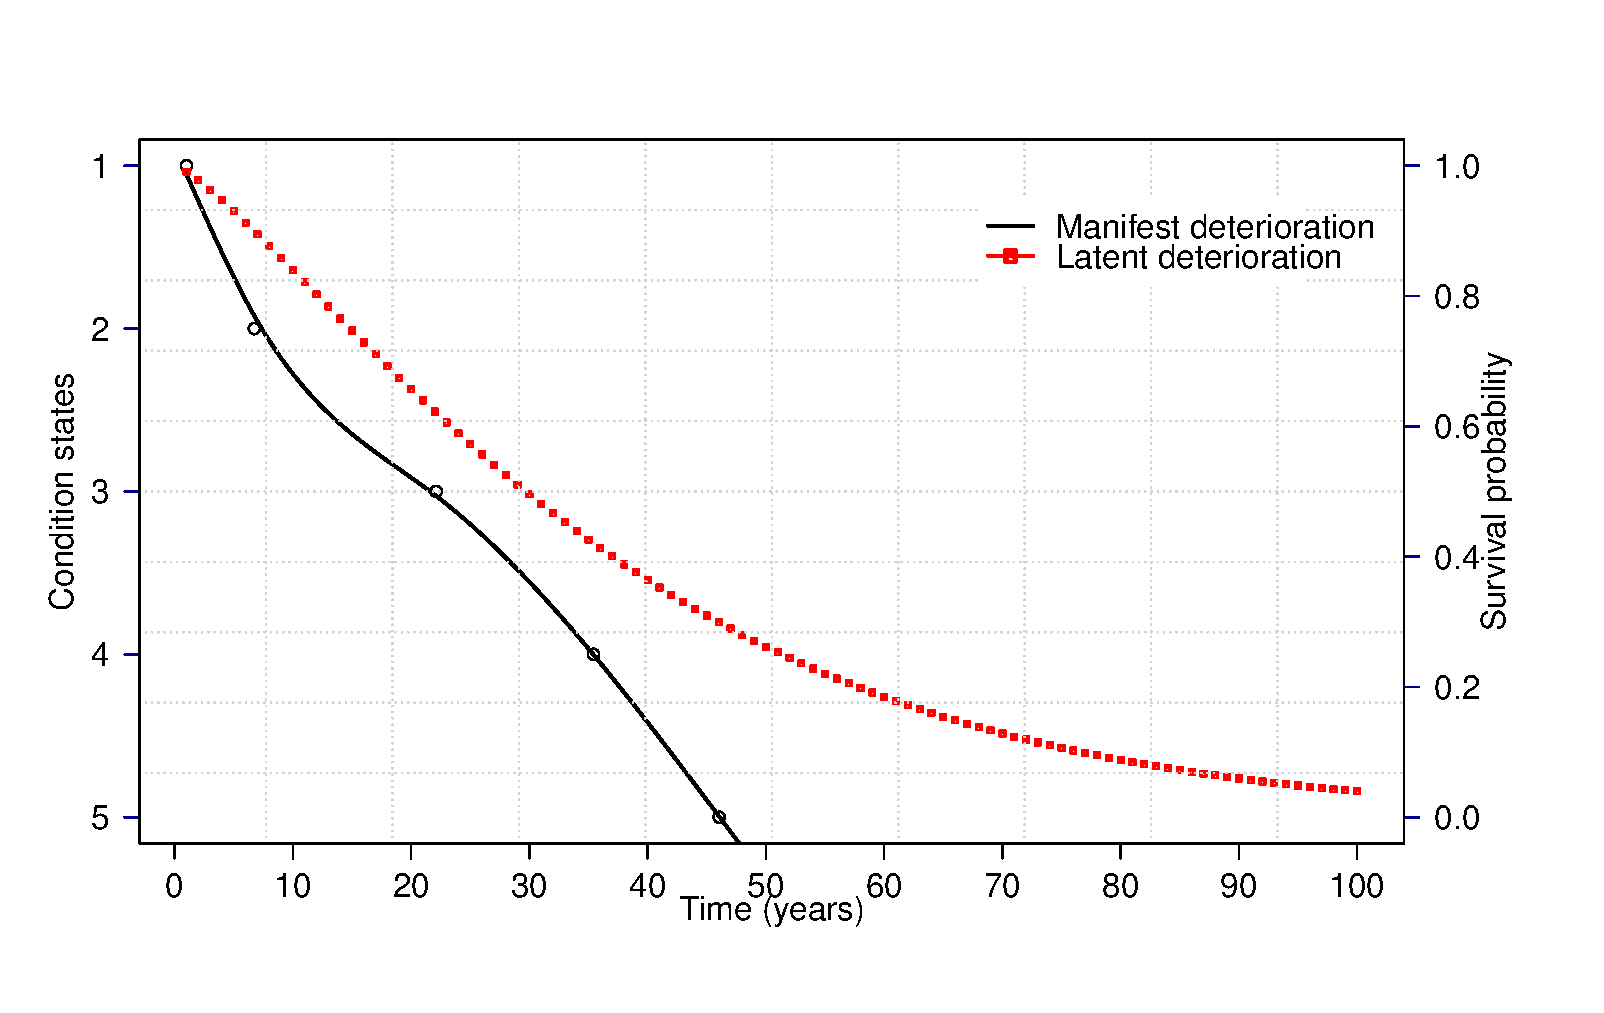
\includegraphics[width=0.8\linewidth]{fig1}
%\caption{ Example of a snow barrier system}
%\label{snowbarriers} 
%\end{figure}
In order to minimize such as risk that the snow barrier system fails
due to heavy snow packs formed in the avalanche starting zones, the
system of snow barriers needs to be replaced with an PI after a certain
period of time in service. In this example, an PI for the snow barriers
system is a replacement of the old system with a new identical one.
In between two consecutive executions of PIs, if the snow barriers
system fails and avalanche occur, immediately after that and CI needs
to be executed. It is considered that the CI for the snow barriers
system is also the replacement of the old one with a new system. However,
as it is executed unexpectedly, the impacts incurred during the execution
of an CI will be higher than that of the PI.

Without loss of generality, it is assumed that the PI ($c_1$) costs 1 monetary
unit (mu). The impacts of the CIs on the snow-barrier system ($c_2$) are 2
mus and on the bridge ($w$) are 10 mus, respectively. Values of $c_3$ and $k_0$ are assumed to be 0 as they can be omitted in the equation (\ref{omegaPI3}) for simplicity but still without loss of generality. It is important to
noted here that these impacts can be separated into two parts. One
is the impact due to avalanches before the execution of the CI and
the other is impact during the execution of the CI. It is important
at this outset of the calculation to mention that it is not necessary
to demonstrate the usefulness of the model with a real case study
since, from mathematical point of view, the determination of the optimal
replacement time (ORT) is dependent mainly on the ratio between
the PI and CI once the reliability of the APS and the protected structure are determined.
The the optimal replacement time were investigated to be every year
to every 50 years, with one year increments 
\subsection{Probable states of the snow barrier system}
The probability of the snow barrier system being in the failure state
is estimated with a Weibull function as described in sub-section \ref{apsrel}.
Values of $\xi$ and $m$ are $0.0252$ and $1.2665$, respectively. With
these values, once can construct the reliability curves as shown in
Figure \ref{reliability-snowbarriers}.

\begin{figure}[H]
\centering{}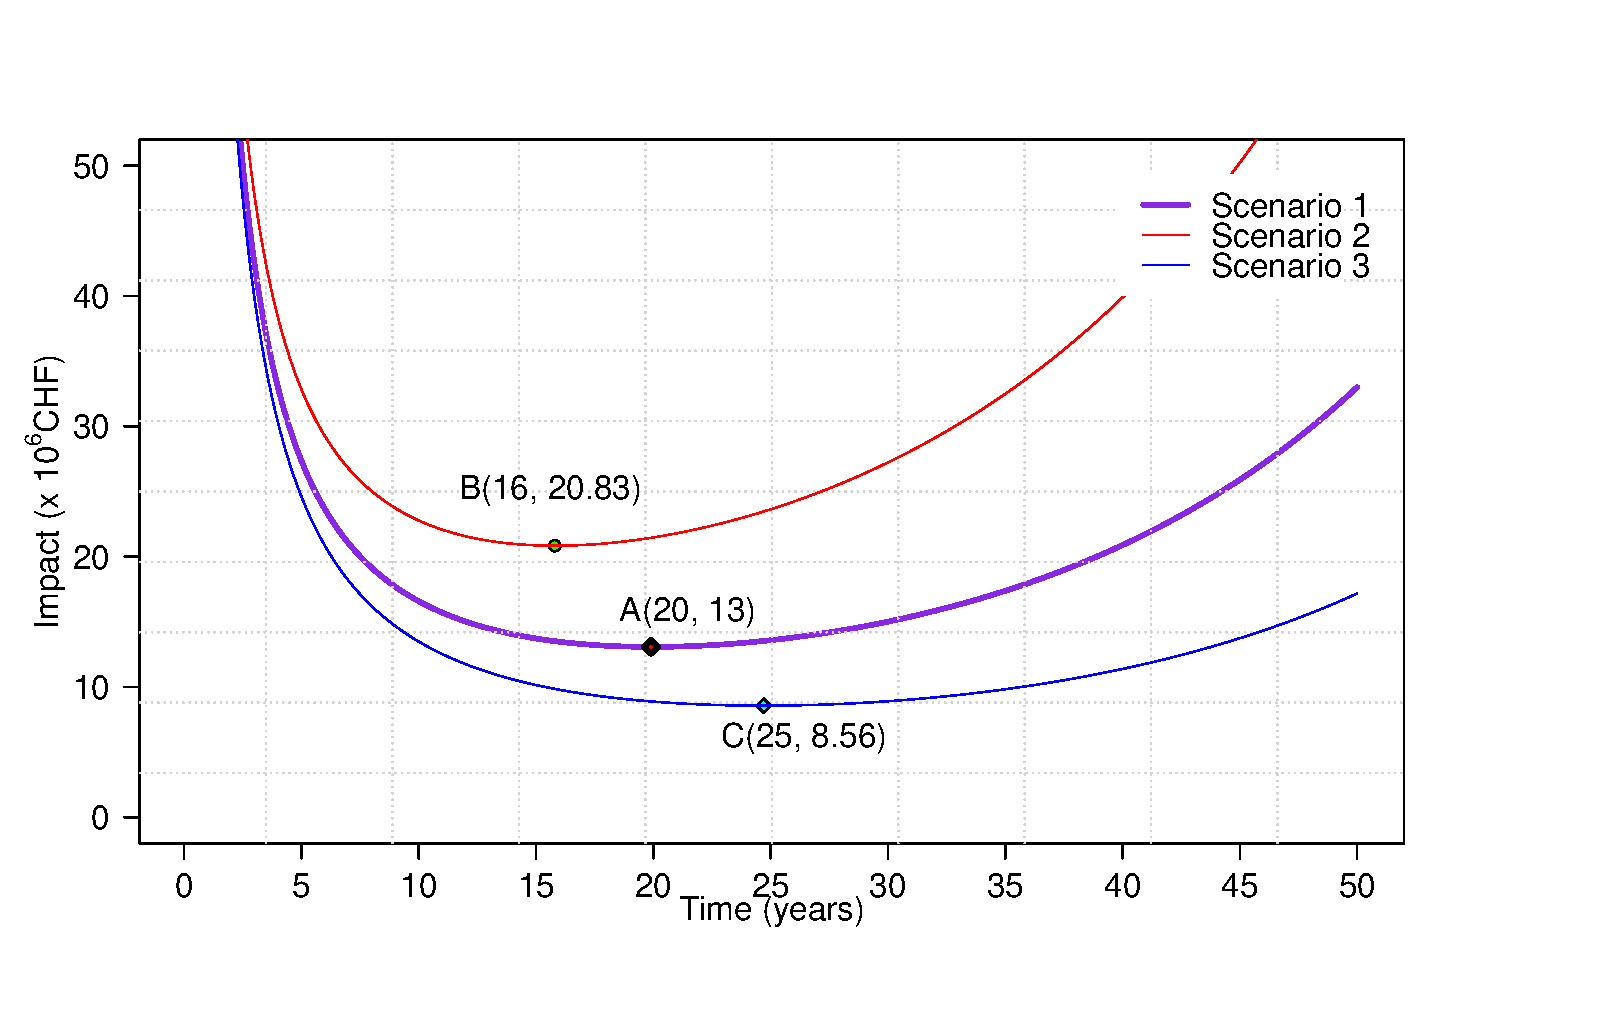
\includegraphics[width=0.8\linewidth]{fig2}
\caption{Probable of snow-barrier system being in the failure state}
\label{reliability-snowbarriers} 
\end{figure}

The reliability curves shows a gradual decrease in the reliability
of the snow-barrier system over time. More or less after 25 years,
the reliability of the system will reduce to about 50\%.

\subsection{Probable states of the bridge}

The probable states of the bridge are estimated using Eq.
(\ref{mtp-1}) and Eqs. (\ref{fragility1-1}), (\ref{fragility2-1}),
and \ref{fragility3-1}. The five non-failure states and the failure
state of the bridge are defined based as shown in Table \ref{statedefinition}.

\begin{table}[H]
\caption{Bridge states (Adapted from \citep{Lethanh2015})}


\begin{centering}
\begin{tabular}{p{2cm}|p{1cm}|p{1.5cm}|l|p{6cm}}
\hline 
\multicolumn{1}{c|}{State} & \multicolumn{2}{c|}{Level of service (LOS)} & \multicolumn{1}{c|}{State} & \multicolumn{1}{c}{Definition}\tabularnewline
\cline{2-3} \cline{5-5} 
\multicolumn{1}{c|}{} & \multicolumn{1}{c|}{Number} & \multicolumn{1}{c|}{Description} & \multicolumn{1}{c|}{} & \tabularnewline
\hline 
\multicolumn{1}{c|}{non-failure} & \multicolumn{1}{c|}{0} & \multicolumn{1}{c|}{Full service} & \multicolumn{1}{c|}{$i=1$} & Deck is new or near new, almost no sign of deterioration \tabularnewline
\cline{4-5} 
\multicolumn{1}{c|}{} & \multicolumn{1}{c|}{} & \multicolumn{1}{c|}{} & \multicolumn{1}{c|}{$i=2$} & Leakage is occurring over $<10\%$ of deck surface area \tabularnewline
\cline{4-5} 
\multicolumn{1}{c|}{} & \multicolumn{1}{c|}{} & \multicolumn{1}{c|}{} & \multicolumn{1}{c|}{$i=3$} & Leakage is occurring over $<25\%$ of deck surface area \tabularnewline
\cline{4-5} 
\multicolumn{1}{c|}{} & \multicolumn{1}{c|}{} & \multicolumn{1}{c|}{} & \multicolumn{1}{c|}{$i=4$} & Leakage is occurring over $\ge25\%$ of deck surface are, some spalling
is occurring, substantial efflorescence, \tabularnewline
\cline{4-5} 
\multicolumn{1}{c|}{} & \multicolumn{1}{c|}{} & \multicolumn{1}{c|}{} & \multicolumn{1}{c|}{$i=5$} & Heavy spalling, heavy efflorescence, deck saturated to point that
concrete is rubble \tabularnewline
\hline 
\multicolumn{1}{c|}{failure} & \multicolumn{1}{c|}{1} & \multicolumn{1}{c|}{No service} & \multicolumn{1}{c|}{$l=1$} & the bridge is not usable \tabularnewline
\hline 
\end{tabular}
\par\end{centering}

\label{statedefinition} 
\end{table}

The transition probabilities between non-failure states for 1 year
($z=1$) are estimated from the values of hazard rates, which are
$\theta_{i}=(0.06,0.09,0.19,0.25,0)$. Table \ref{transitionmatrixa}
shows the values of each transition probability.

\begin{table}[H]
\caption{Transition probabilities between non-failure states for the bridge
excluding the probability of failure}
\begin{centering}
\begin{tabular}{l|l|lllll}
\hline 
\multicolumn{1}{l}{} & \multicolumn{6}{c}{Year ($t+1$)}\tabularnewline
\hline 
 & non-failure states  & $i=1$  & $i=2$  & $i=3$  & $i=4$  & $i=5$ \tabularnewline
\hline 
 & $i=1$  & 0.94176  & 0.05567  & 0.00241  & 0.00015  & 0.00001 \tabularnewline
 & $i=2$  & 0  & 0.91393  & 0.07827  & 0.00717  & 0.00062 \tabularnewline
 & $i=3$  & 0  & 0  & 0.82696  & 0.15250  & 0.02054 \tabularnewline
 & $i=4$  & 0  & 0  & 0  & 0.77880  & 0.22120 \tabularnewline
\begin{rotate}{90} Year ($t$) \end{rotate}  & $i=5$  & 0  & 0  & 0  & 0  & 1 \tabularnewline
\hline 
\end{tabular}
\par\end{centering}
\label{transitionmatrixa} 
\end{table}
The transition probabilities between non-failure states and the failure
state, and the the parameter values of $\delta$ and $\gamma$ are
given in (Table \ref{alphagammavalue}). The parameter values are used for illustrative purposes, but they can be calculated using the methodology presented in \citet{Schultz2010}. 
\begin{table}[H]
\caption{Transition from non-failure states to the failure state}
\begin{centering}
\begin{tabular}{l|l|l|l}
\hline 
\multicolumn{1}{c|}{Non-failure state} & \multicolumn{2}{c|}{Failure state ($l=1$)} & Transition probability\tabularnewline
\cline{2-4} 
\multicolumn{1}{c|}{} & $\delta$  & $\gamma$  & $p_{il}$\tabularnewline
\hline 
\multicolumn{1}{c|}{$i=1$} & \multicolumn{1}{c|}{0.353} & \multicolumn{1}{c|}{5.652} & 0.00024 \tabularnewline
\hline 
\multicolumn{1}{c|}{$i=2$} & \multicolumn{1}{c|}{0.360} & \multicolumn{1}{c|}{5.581} & 0.00071 \tabularnewline
\hline 
\multicolumn{1}{c|}{$i=3$} & \multicolumn{1}{c|}{0.371} & \multicolumn{1}{c|}{5.575} & 0.00157 \tabularnewline
\hline 
\multicolumn{1}{c|}{$i=4$} & \multicolumn{1}{c|}{0.389} & \multicolumn{1}{c|}{5.498} & 0.00679 \tabularnewline
\hline 
\multicolumn{1}{c|}{$i=5$} & \multicolumn{1}{c|}{0.391} & \multicolumn{1}{c|}{5.367} & 0.01366 \tabularnewline
\hline 
\end{tabular}
\par\end{centering}
\label{alphagammavalue} 
\end{table}

The last column of Table \ref{alphagammavalue} shows the probability
of transitioning from a non-failure state to a failure state. The
values were calculated for one year transition. It can be seen that
there is an increasing probability of transition with an increasingly
poor non-failure state. Using equation \ref{delta-1}, the transition
probabilities between non-failure states were adjusted to take into
consideration the probability of being in a failure state (Table \ref{totalmatrix}).
\begin{table}[H]
\caption{Complete transition probability matrix}
\begin{centering}
\begin{tabular}{l|l|lllll|l}
\hline 
\multicolumn{1}{l}{} & \multicolumn{7}{c}{Year ($t+1$)}\tabularnewline
\cline{2-8} 
\multicolumn{1}{l|}{} & State  & $i=1$  & $i=2$  & $i=3$  & $i=4$  & $i=5$  & $l=1$ \tabularnewline
\hline 
 & $i=1$  & 0.94154  & 0.05565  & 0.00241  & 0.00015  & 0.00001  & 0.00024 \tabularnewline
 & $i=2$  & 0  & 0.913288  & 0.07822  & 0.00716  & 0.00062  & 0.00071 \tabularnewline
 & $i=3$  & 0  & 0  & 0.82566  & 0.15226  & 0.02051  & 0.00157 \tabularnewline
 & $i=4$  & 0  & 0  & 0  & 0.77352  & 0.21970  & 0.00679 \tabularnewline
\begin{rotate}{90} Year ($t$) \end{rotate}  & $i=5$  & 0  & 0  & 0  & 0  & 0.98634  & 0.01366 \tabularnewline
\hline 
 & $l=1$  & 0  & 0  & 0  & 0  & 0  & 1 \tabularnewline
\hline 
\end{tabular}
\par\end{centering}
\label{totalmatrix} 
\end{table}


%%%%%%%%%%%%%%%Evolution of condition states
The predicted evolution of the state of the bridge from its initial
state $\pi_{i}=(1,0,0,0,0)$ over a period of 50 years is given in
Figure \ref{csevolution}.
\begin{figure}[H]
\centering{}\includegraphics[width=1\linewidth]{fig3} \caption{Predicted evolution of the state of the bridge }
\label{csevolution} 
\end{figure}
%In Figure \ref{csevolution}, the black proportion represents the probability of being the failure state ( $l=1$). %The multiplication of the state probabilities ($\pi{}_{l}^{k}(t)$ in Eq. (\ref{totalCIs}), $k=1$ as there is only one bridge) and the unit impact ($Y=10$) mus of the CI for the bridge gives the expected total impact for the bridge in the respective year. This value will be a part of total CI shown in Eq. (\ref{totalCIs}). %%%%
\subsection{Determination of optimal replacement time}
With the information given in the previous sections, the model given
in section \ref{model} was used to estimate the total impacts associated with
the investigated replacement strategies for the APS within a 50 year
period. The results are shown in red curve in Figure \ref{results}.
At every point of the curve, the corresponding value to the vertical
axis is the cumulative impacts over the 50 years if the preventive
intervention is executed repeatably at the time corresponding to the
value of the horizontal axis.

\begin{figure}[H]
\centering{}\includegraphics[width=0.8\linewidth]{fig4}
\caption{Impacts for investigated replacement strategies}
\label{results} 
\end{figure}

It can be seen that the optimal time to execute a PI is every 19 years
(point A) because this will result in an total impact will be minimal
($6.59$ $mus$). If either the PI is executed before or after that
time, the impact will be higher. This is because if the PI is done
earlier or more frequent, the impacts of executing PI will exponentially
increase, and if the PI is executed less frequently, the impacts incurred
by executing CIs will exponentially increase. 

\section{Sensitivity analysis}
\label{sa} As there are high levels of uncertainty often associated
with the values of impacts and in the parameters used in the estimation
of the probability of failure of the APS a sensitivity analysis was
conducted to explore the effect on that variations in these values
has on the optimal replacement strategy. The range of values investigated
are shown in Table \ref{sensi1}. 

\begin{table}[h]
\begin{centering}
\caption{Range of values used in the sensitivity analysis}
\begin{tabular}{l|c|cc}
\hline 
\multirow{2}{*}{Criteria}  & \multirow{2}{*}{Notation}  & \multicolumn{2}{c}{Range of value}\tabularnewline
%\hline 
 &  & \multicolumn{1}{l|}{Min} & \multicolumn{1}{l}{Max}\tabularnewline
\hline 
\multirow{2}{*}{Impact ratio}  & $c_2$  & \multicolumn{1}{c}{0.1} & 10 \tabularnewline
%\hline 
 & $w$  & \multicolumn{1}{c}{0.1} & 1'000 \tabularnewline
\hline 
\multirow{2}{*}{%
\begin{tabular}{@{}l@{}}
Reliability of\tabularnewline
snow-barrier system\tabularnewline
\end{tabular}}  & $\xi$  & \multicolumn{1}{c}{0.001} & 0.1 \tabularnewline
\hline 
 & $m$  & \multicolumn{1}{c}{1} & 3 \tabularnewline
\hline 
\multirow{2}{*}{%
\begin{tabular}{@{}l@{}}
Reliability of\tabularnewline
bridge\tabularnewline
\end{tabular}}  & 100\% in state  & \multicolumn{1}{c}{1} & 5 \tabularnewline
\hline 
 & Avalanche intensity ($m^{3}$)  & \multicolumn{1}{c}{1} & 20 \tabularnewline
\hline 
Discount factor (\%)  & $\alpha$  & \multicolumn{1}{c}{0} & 10 \tabularnewline
\hline 
\end{tabular}
\par\end{centering}
\centering{}
\label{sensi1} 
\end{table}

\begin{figure}[H]
\centering{}\includegraphics[width=0.8\linewidth]{fig5} \caption{Optimal replacement time in 50 years}
\label{results-1} 
\end{figure}
Also in Figure \ref{results-1}, there are purple curve and blue curve,
which are drawn by selecting the value of impact for a CI for the
snow-barriers system to be double and half of that used in the reference
case, respectively. The purpose is to demonstrate the changes in the
optimal time to execute an PI on the snow barriers system when there
are changes in the impacts related to CIs of the bridge. It can be
concluded that increases in the impact of a CI on the bridge the more
frequent PI on the snow barriers system should be executed, and vice-versa.
The following section gives an in-depth sensitivity analysis on the
change in the ratio between the value of the impacts of the PI of
the snow barriers system and CI on the bridge, as well as on the change
of parameters used in the model. 

%In the table, the notation $CI_{A}$ and $CI_{B}$ are used for impacts
%related to CIs of the snow barriers system and the bridge, respectively.
The results of the SA for the value of impacts $c_2$ and $w$ are shown in graphs
of Figure \ref{impactratio}.

\begin{figure}[ht!]
\centering{}\subfigure[$c_2$]{ \includegraphics[width=0.45\linewidth]{fig6a}
} \subfigure[$w$]{\includegraphics[width=0.45\linewidth]{fig6b}
} \caption{SA-impact ratio}
\label{impactratio} 
\end{figure}

\begin{figure}[ht!]
\centering{}\subfigure[$\xi$]{ \includegraphics[width=0.45\linewidth]{fig7a}
} \subfigure[$m$]{ \includegraphics[width=0.45\linewidth]{fig7b} }
\caption{SA-reliability of the snow-barrier system}
\label{reliabilitySPS} 
\end{figure}

\begin{figure}[ht!]
\centering{}\subfigure[Avalanche intensity]{ \includegraphics[width=0.45\linewidth]{fig8a}
} \subfigure[Age of bridge]{\includegraphics[width=0.45\linewidth]{fig8b}} \caption{SA-Avalanche intensity and state of the bridge}
\label{reliabilitybridge} 
\end{figure}


\begin{figure}[ht!]
%\subfigure[Discount factor]%	{

\centering{}\includegraphics[width=0.45\linewidth]{fig9} % }
\caption{SA-Discount factor}
\label{SAdiscount} 
\end{figure}

Following conclusions can be drawn by interpreting the changes in the
optimal time to execute the PI with respect to different criteria
\begin{itemize}
\item The lower the value of $c_2$, is, the longer the optimal
replacement time (ORT) becomes (Figure \ref{impactratio}). The ORT
is quite sensitive to the value of $c_2$, but not so
sensitive to the value of $w$. This is because the
impacts incurred by executing the CI for the snow-barriers system
will dramatically change the reliability of the system itself. Whilst,
the value of $w$ has to be multiplied with the transition
probability of the latent state of the bridge, which is in fact significantly
low in this example (Table \ref{totalmatrix} and Figure \ref{csevolution}), 
\item The ORT depends greatly on the values of parameters of the reliability
function used for the snow-barrier system. As can be seen from Figure
\ref{reliabilitySPS}, the ORT decreases nonlinearly as values of $\xi$
and $m$ increases. In the case of Weibull function, if value of $\xi$
and $m$ increases, it means the rate of failure increases and therefore
it is better to execute the PI earlier, 
\item The intensity of avalanche $s$ has a great influence on both the ORT and
the total impacts (Figure \ref{reliabilitybridge}-a) when it reaches
to a certain threshold. For example, when the intensity of avalanche
becomes more than 10 $m^{3}$, there is a sharp decreasing in the
ORT and a sharp increasing in the value of impact. This is because,
the bridge itself was designed to withstand a certain intensity of
avalanche. However, if the intensity of avalanche reaches to a certain
level, there is a higher chance that the bridge will be in adequate
level of service. Under this circumstance, the value of CI on the
bridge will plays an important part in determining the ORT. This finding
is important for manager to carefully use the fragility curve for
their objects by examining the most likely values of parameters of
the fragility curves (e.g. values of $\delta$ and $\gamma$ in Eq.
(\ref{fragility3-1})), 
\item The ORT depends also on actual state probability of the bridge. This
conclusion can be confirmed with the curves shown in Figure \ref{reliabilitybridge}-b.
The ORT tends is shorter when the state of the bridge gets worse (e.g.
from being in state 1 to state 5). In this figure, the changes is
not significant. However, it is not because the values of the state
probability of the bridge but it is because the transition probability
from non-failure state to failure state is really small. This is an
interesting finding and convey an implication that managers, when
determining the ORT for the snow-barrier system, they have to take
into consideration of how the actual condition of other objects that
being affected by the avalanche (e.g. the bridge), 
\item Changes in value of the discount factor is quite sensible to the change
in the impact. However, it does not significantly change the value
of ORT. In this example, the values of the discount factor was varied
from 0 to 10\%, however, the difference of the ORT is only 4 years
(Figure \ref{SAdiscount}). This is also an interesting point when
managers consider to manage both the snow-barriers system and the
bridge in a infinite time (e.g. long term management). Under an infinite
case, the values of discount factor can be close to 0 (e.g. interest
rate in developed nations is extremely small) or even can be ignored
from the mathematical view points. This will make the numerical solution
to the model more convenient. 
\end{itemize}

\section{Conclusion}

\label{conclusion} In this paper, a two state time-dependent
replacement model, which can be used to determine the optimal time
to execute a preventive intervention for avalanche protection structures,
is presented. The methodology is composed of an extended time-dependent
replacement model that can take into consideration of infinite time horizon and impacts incurred during the preventive
intervention and corrective intervention of the avalanche protection
structures and the impacts incurred if the critical structures fail
to provide adequate level of services one avalanche hit them. It also
includes the discussion on the integration of existing fragility curves
and Markov model used to model the manifest and latent deterioration
of civil structures that could be in state of failure due to avalanche.

A numerical example was conducted for a snow-barriers system, which
was installed in the starting zones of avalanche. The reliability
of the system decreases over time and might fails to against avalanche.
Consequently, avalanche might come into contact with a bridge and
cause the bridge to be in inadequate level of service. Results of
the example highlight important message to infrastructure managers
of the avalanche protection system that the system should be replaced
at an optimal time in order to minimize all negative impacts incurred
by the stakeholders. The determination of the time is crucially dependent
on the ratio of the impacts between the corrective intervention and
preventive intervention as well as on the parameter values used to
represent the reliability of the snow-barriers system. Future expansion of the model should consider also the joint preventive intervention plan for both the avalanche protection structure and the protected structure.


%\begin{verbatim}
\bibliographystyle{apa}
%\renewcommand\bibliographytypesize{\fontsize{10}{12}\selectfont}
\bibliography{nSIEguide}
%\end{verbatim}

\end{document}
